\section{Полученные результаты}

\subsection{Расчёт многослойной преграды}
При расчёте задачи о непробивающем ударе по многослойной преграде использовались
данные из табл. \ref{tbl:subpackage}. В табл. \ref{tbl:subpackage_2} приведены
безразмерные величины, использовавшиеся в расчёте.
\begin{table}[h]
\centering
\begin{tabular}{|c|c|c|c|}
\hline
Слой & $\rho$ & $\lambda$ & $\mu$  \\
\hline
Эпоксидная смола & 1.25 & 1440 & 960 \\
Субпакет & 1.25 & 4620 & 3080 \\
\hline
\end{tabular}
\caption{Безразмерные характеристики слоёв.}
\label{tbl:subpackage_2}
\end{table}

Давление в зоне воздействия ударника задавалось равным 50 МПа (50 единиц в безразмерных величинах).

На графиках (см. рис. \ref{pic:multilayer_init}-\ref{pic:multilayer_Rayleigh_2})
изображены результаты численного расчёта задачи.
На рис. \ref{pic:multilayer_b1}-\ref{pic:multilayer_b3} изображен процесс
прохождения волны через границы раздела двух слоёв. Несмотря на то, что
конструкция состоит из пяти слоёв, волновая картина имеет весьма сложный
вид. На рис. \ref{pic:multilayer_b1}-\ref{pic:multilayer_b3} видны различные
виды волн: волна, созданная начальным возмущением, отраженные от границ волны и
волны, распространяющиеся вдоль границы раздела. Последние, так называемые волны
Рэлея (см. рис. \ref{pic:multilayer_Rayleigh_1}-\ref{pic:multilayer_Rayleigh_2}), 
представляют особый интерес. Появление таких волн в композитных материалах
ожидаемо, но аналитических расчётов, подтверждающих их наличие, на данный момент
нет. Рэлеевские волны формируются на границе раздела двух неоднородных сред и
распространяются вдоль этой границы. Такие волны можно наблюдать, например, в фундаментах
зданий во время землетрясений. Из-за своей низкой частоты, большой
амплитуды и длительного воздействия именно рэлеевские волны наносят наибольший
ущерб зданиям после сейсмической активности. Обнаружение этих волн в композитных
материалах позволяет сделать предположение о том, что области наибольших
напряжений, а, следовательно, и области потери прочности будут сосредоточены
вдоль границ раздела слоёв.

Полученные результаты численного моделирования хорошо согласуются с теоретическими данными,
а также интересны с практической точки зрения. В связи с этим 
дальнейшее исследование волновой картины в композиционных
материалах описанным в работе методом представляет серьёзный научный интерес,
так как может дать ответ на вопрос о том, как ведут себя такие материалы при
непробивающих ударах.
\begin{figure}[htp]
\centering
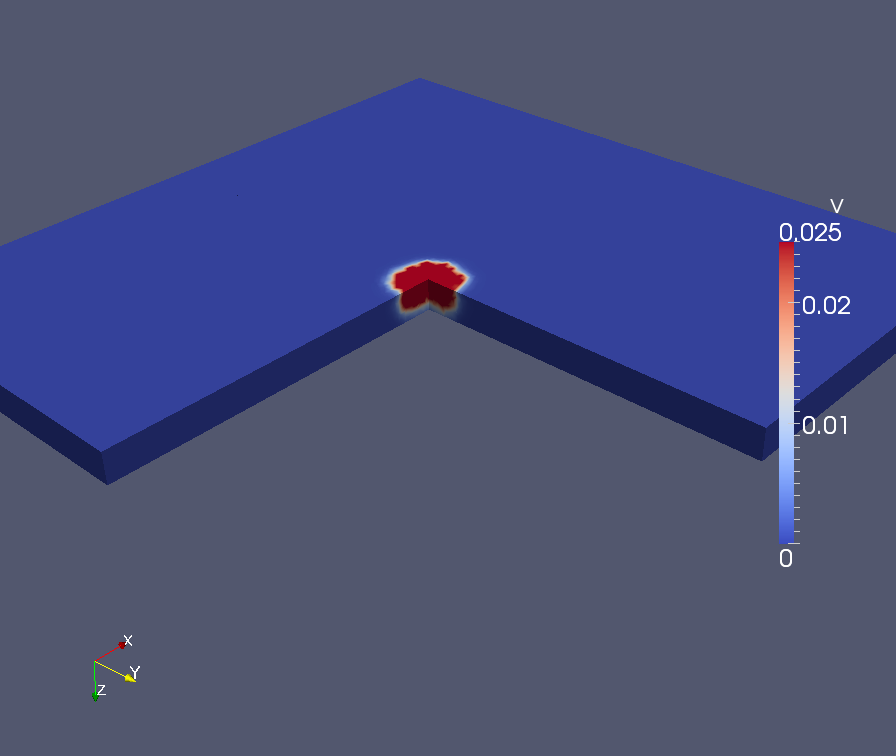
\includegraphics[width=\textwidth]{png/v-0001.png}
\caption{Начальное возмущение. На рисунке цветом изображены модули скоростей в
двух взаимно перпендикулярных срезах.}
\label{pic:multilayer_init}
\end{figure}
\begin{figure}[htp]
\centering
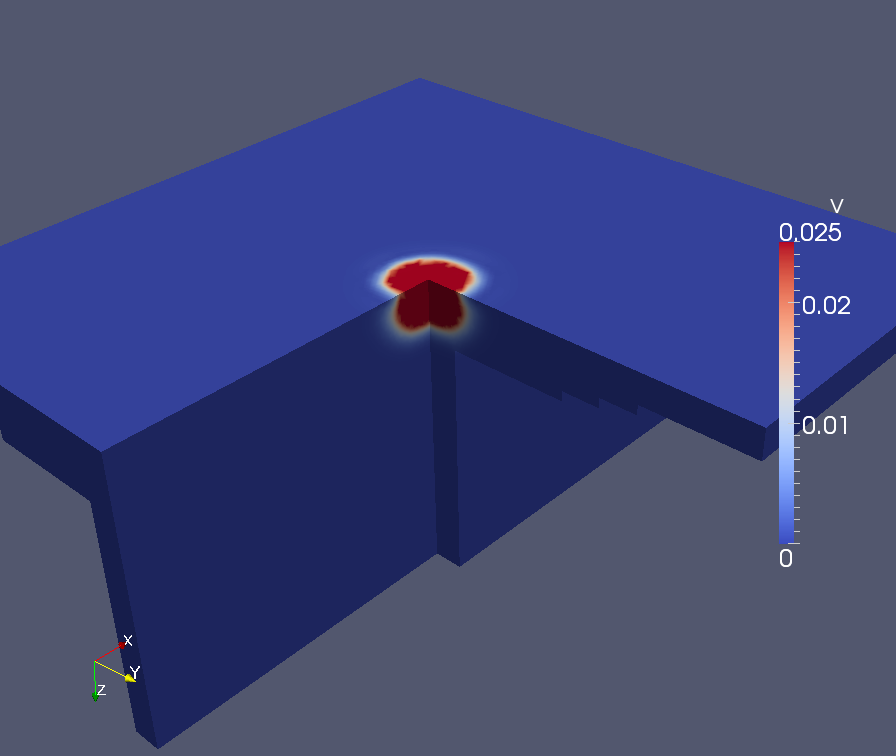
\includegraphics[width=\textwidth]{png/v-0003.png}
\caption{Отражение от первой границы. На рисунке цветом изображены модули скоростей в
двух взаимно перпендикулярных срезах.}
\label{pic:multilayer_b1}
\end{figure}
\begin{figure}[htp]
\centering
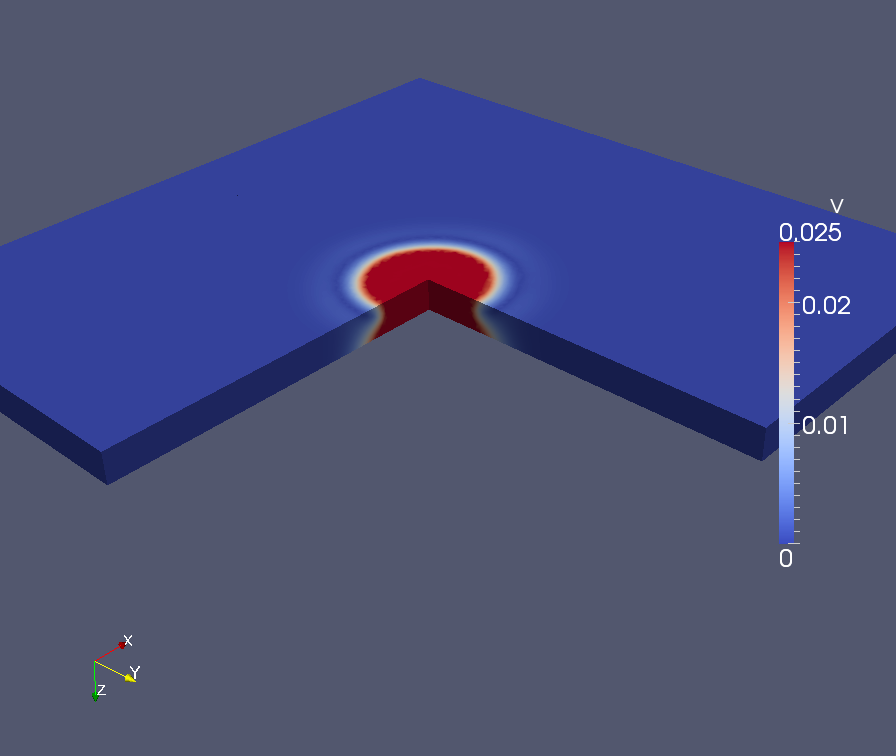
\includegraphics[width=\textwidth]{png/v-0007.png}
\caption{Отражение от второй границы. На рисунке цветом изображены модули скоростей в
двух взаимно перпендикулярных срезах.}
\label{pic:multilayer_b2}
\end{figure}
\begin{figure}[htp]
\centering
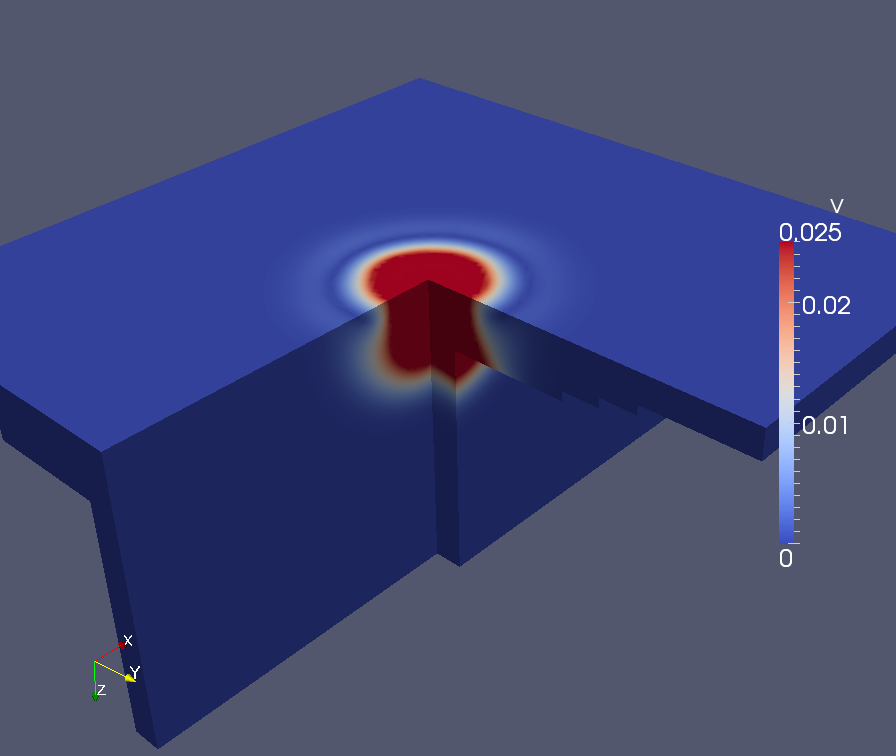
\includegraphics[width=\textwidth]{png/v-0009.png}
\caption{Отражение от третьей границы. На рисунке цветом изображены модули скоростей в
двух взаимно перпендикулярных срезах.}
\label{pic:multilayer_b3}
\end{figure}
\begin{figure}[htp]
\centering
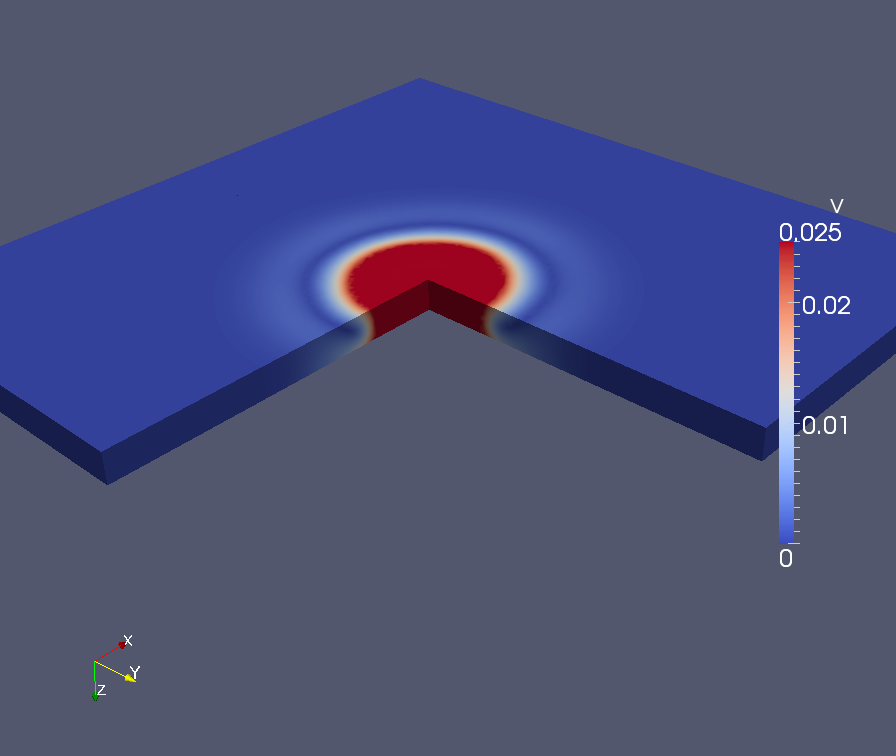
\includegraphics[width=\textwidth]{png/v-0013.png}
\caption{Формирование волны Рэлея. На рисунке цветом изображены модули скоростей
в срезе, перпендикулярном оси x, а стрелками обозначены поля скоростей.}
\label{pic:multilayer_Rayleigh_1}
\end{figure}
\begin{figure}[htp]
\centering
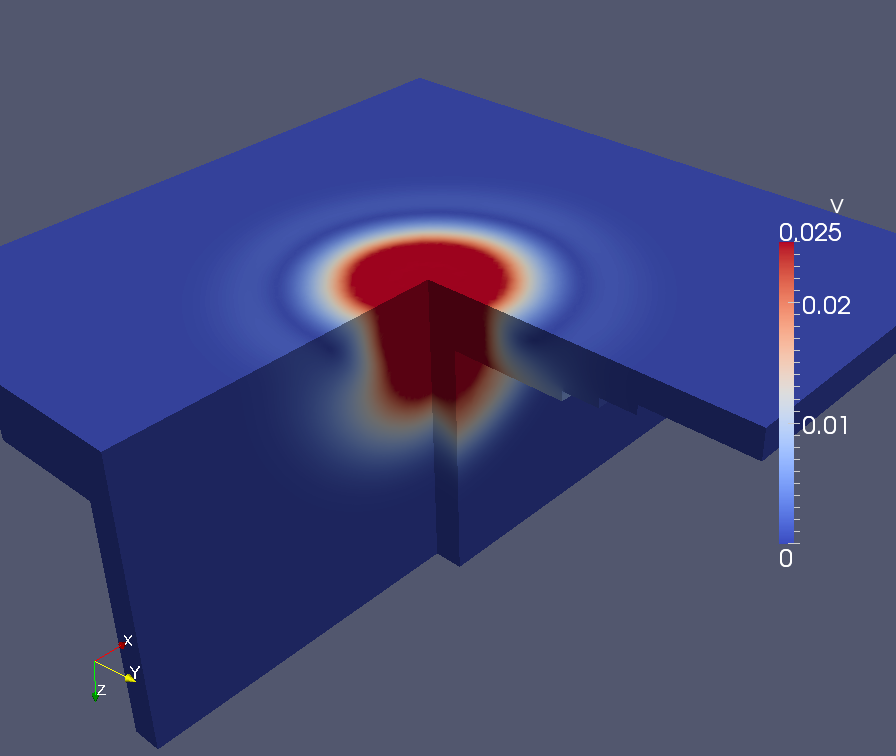
\includegraphics[width=\textwidth]{png/v-0016.png}
\caption{Распространение волны Рэлея. На рисунке цветом изображены модули скоростей
в срезе, перпендикулярном оси x, а стрелками обозначены поля скоростей.}
\label{pic:multilayer_Rayleigh_2}
\end{figure}
